\documentclass{article}
\usepackage{helvet}
\renewcommand{\familydefault}{\sfdefault}
\usepackage{graphicx}
\usepackage{geometry}
\geometry{a4paper, margin=1in}
\title{Report Assignment 2: Microservices}
\author{Yonah Thienpont}
\date{\today}

\begin{document}

\maketitle

\section{Microservices Decomposition}
The application is decomposed into the following microservices:
\begin{itemize}
    \item \textbf{Authentication Service}
    \item \textbf{Event Service}
    \item \textbf{Calendar Service}
\end{itemize}
Each microservice has their own database called 'auth-db', 'event-db' and 'cal-db', respectively.

\subsection{Authentication Service}
\begin{itemize}
    \item \textbf{Features}: User registration, login, and user information retrieval.
    \item \textbf{Data}: Stores user credentials and profile information.
    \item \textbf{Connections}: Returns whether a user exists to the calendar services, when we try to share a calendar with a non-existing user.
\end{itemize}

\subsection{Event Service}
\begin{itemize}
    \item \textbf{Features}: Create events, view event details, list public events, manage RSVPs, and fetch user-specific events.
    \item \textbf{Data}: Stores event details and RSVP statuses.
    \item \textbf{Connections}: Retrieves user information from the Authentication Service and integrates with the Calendar Service to display events.
\end{itemize}

\subsection{Calendar Service}
\begin{itemize}
    \item \textbf{Features}: Share calendar, view shared calendars, and list user-specific events.
    \item \textbf{Data}: Manages shared calendar relationships.
    \item \textbf{Connections}: Interacts with the Authentication Service to verify users and with the Event Service to fetch event data.
\end{itemize}

\begin{figure}[h!]
    \centering
    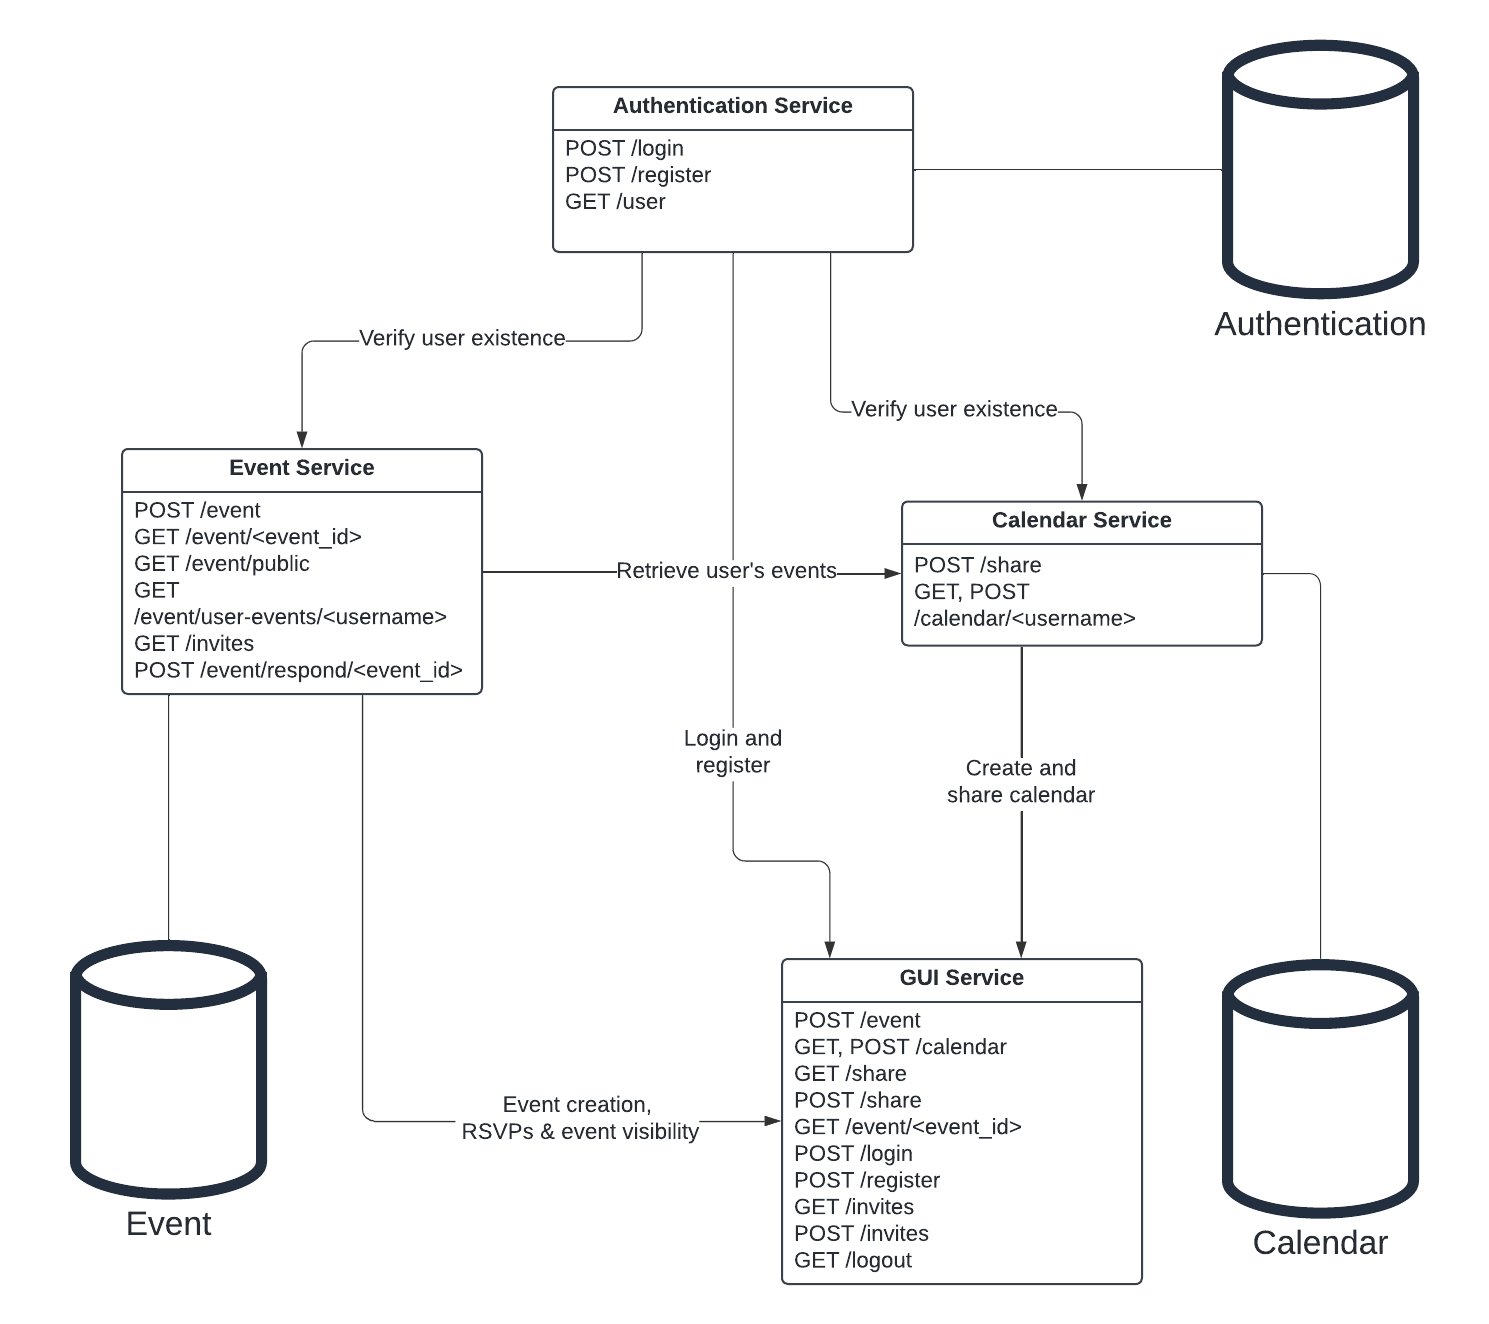
\includegraphics[width=\textwidth]{Microservices.png}
    \caption{Overview of the Microservice Architecture}
    \label{fig:architecture}
\end{figure}

\section{Explanation of Decomposition}
\subsection{Grouping of Features}
Features were grouped based on their core functionalities:
\begin{itemize}
    \item \textbf{Authentication}: Handles user-related operations like registration and login.
    \item \textbf{Event Management}: Manages event creation, RSVPs, and event visibility.
    \item \textbf{Calendar Management}: Deals with personal and shared calendars.
\end{itemize}

\subsection{Consequences of Service Failures}
\begin{itemize}
    \item \textbf{Authentication Service Failure}: Users cannot log in or register, affecting overall access.
    \item \textbf{Event Service Failure}: Users cannot create or respond to events, affecting event-related activities.
    \item \textbf{Calendar Service Failure}: Users cannot view or share calendars, affecting calendar visibility.
\end{itemize}

\subsection{Scalability}
The approach allows each service to scale independently based on demand:
\begin{itemize}
    \item \textbf{Authentication Service}: Can be scaled to handle high login/register traffic.
    \item \textbf{Event Service}: Can be scaled to manage numerous event-related operations.
    \item \textbf{Calendar Service}: Can be scaled to support extensive calendar interactions.
\end{itemize}

\section{Bugs}
When responding to an event, you will have to refresh the page manually to see the change take effect. The API calls and their statuses are correct.

\section{Implementation}
Below are the API endpoints for each required feature:

\subsection{Authentication Service}
\begin{itemize}
    \item \textbf{Login}
    \begin{verbatim}
    POST /login
    \end{verbatim}
    \item \textbf{Register}
    \begin{verbatim}
    POST /register
    \end{verbatim}
    \item \textbf{Get User}
    \begin{verbatim}
    GET /user/{username}
    \end{verbatim}
\end{itemize}

\subsection{Event Service}
\begin{itemize}
    \item \textbf{Create Event}
    \begin{verbatim}
    POST /event
    \end{verbatim}
    \item \textbf{View Event}
    \begin{verbatim}
    GET /event/{event_id}
    \end{verbatim}
    \item \textbf{Public Events}
    \begin{verbatim}
    GET /event/public
    \end{verbatim}
    \item \textbf{User Events}
    \begin{verbatim}
    GET /event/user-events/{username}
    \end{verbatim}
    \item \textbf{Pending Invites}
    \begin{verbatim}
    POST /invites
    \end{verbatim}
    \item \textbf{Respond to Invite}
    \begin{verbatim}
    POST /event/respond/{event_id}
    \end{verbatim}
\end{itemize}

\subsection{Calendar Service}
\begin{itemize}
    \item \textbf{Share Calendar}
    \begin{verbatim}
    POST /share
    \end{verbatim}
    \item \textbf{View Calendar}
    \begin{verbatim}
    GET /calendar/{username}
    POST /calendar/{username}
    \end{verbatim}
\end{itemize}

\end{document}
